% Options for packages loaded elsewhere
\PassOptionsToPackage{unicode}{hyperref}
\PassOptionsToPackage{hyphens}{url}
%
\documentclass[
  12pt,
]{article}
\usepackage{amsmath,amssymb}
\usepackage{lmodern}
\usepackage{iftex}
\ifPDFTeX
  \usepackage[T1]{fontenc}
  \usepackage[utf8]{inputenc}
  \usepackage{textcomp} % provide euro and other symbols
\else % if luatex or xetex
  \usepackage{unicode-math}
  \defaultfontfeatures{Scale=MatchLowercase}
  \defaultfontfeatures[\rmfamily]{Ligatures=TeX,Scale=1}
\fi
% Use upquote if available, for straight quotes in verbatim environments
\IfFileExists{upquote.sty}{\usepackage{upquote}}{}
\IfFileExists{microtype.sty}{% use microtype if available
  \usepackage[]{microtype}
  \UseMicrotypeSet[protrusion]{basicmath} % disable protrusion for tt fonts
}{}
\makeatletter
\@ifundefined{KOMAClassName}{% if non-KOMA class
  \IfFileExists{parskip.sty}{%
    \usepackage{parskip}
  }{% else
    \setlength{\parindent}{0pt}
    \setlength{\parskip}{6pt plus 2pt minus 1pt}}
}{% if KOMA class
  \KOMAoptions{parskip=half}}
\makeatother
\usepackage{xcolor}
\usepackage[margin=1in]{geometry}
\usepackage{longtable,booktabs,array}
\usepackage{calc} % for calculating minipage widths
% Correct order of tables after \paragraph or \subparagraph
\usepackage{etoolbox}
\makeatletter
\patchcmd\longtable{\par}{\if@noskipsec\mbox{}\fi\par}{}{}
\makeatother
% Allow footnotes in longtable head/foot
\IfFileExists{footnotehyper.sty}{\usepackage{footnotehyper}}{\usepackage{footnote}}
\makesavenoteenv{longtable}
\usepackage{graphicx}
\makeatletter
\def\maxwidth{\ifdim\Gin@nat@width>\linewidth\linewidth\else\Gin@nat@width\fi}
\def\maxheight{\ifdim\Gin@nat@height>\textheight\textheight\else\Gin@nat@height\fi}
\makeatother
% Scale images if necessary, so that they will not overflow the page
% margins by default, and it is still possible to overwrite the defaults
% using explicit options in \includegraphics[width, height, ...]{}
\setkeys{Gin}{width=\maxwidth,height=\maxheight,keepaspectratio}
% Set default figure placement to htbp
\makeatletter
\def\fps@figure{htbp}
\makeatother
\setlength{\emergencystretch}{3em} % prevent overfull lines
\providecommand{\tightlist}{%
  \setlength{\itemsep}{0pt}\setlength{\parskip}{0pt}}
\setcounter{secnumdepth}{5}
\newlength{\cslhangindent}
\setlength{\cslhangindent}{1.5em}
\newlength{\csllabelwidth}
\setlength{\csllabelwidth}{3em}
\newlength{\cslentryspacingunit} % times entry-spacing
\setlength{\cslentryspacingunit}{\parskip}
\newenvironment{CSLReferences}[2] % #1 hanging-ident, #2 entry spacing
 {% don't indent paragraphs
  \setlength{\parindent}{0pt}
  % turn on hanging indent if param 1 is 1
  \ifodd #1
  \let\oldpar\par
  \def\par{\hangindent=\cslhangindent\oldpar}
  \fi
  % set entry spacing
  \setlength{\parskip}{#2\cslentryspacingunit}
 }%
 {}
\usepackage{calc}
\newcommand{\CSLBlock}[1]{#1\hfill\break}
\newcommand{\CSLLeftMargin}[1]{\parbox[t]{\csllabelwidth}{#1}}
\newcommand{\CSLRightInline}[1]{\parbox[t]{\linewidth - \csllabelwidth}{#1}\break}
\newcommand{\CSLIndent}[1]{\hspace{\cslhangindent}#1}
\usepackage[left]{lineno}\linenumbers
\usepackage{setspace}\doublespace
\ifLuaTeX
  \usepackage{selnolig}  % disable illegal ligatures
\fi
\IfFileExists{bookmark.sty}{\usepackage{bookmark}}{\usepackage{hyperref}}
\IfFileExists{xurl.sty}{\usepackage{xurl}}{} % add URL line breaks if available
\urlstyle{same} % disable monospaced font for URLs
\hypersetup{
  pdftitle={Mixing cover crops suppresses weeds and roto-till reduces urban soil strength and improves infiltration},
  pdfauthor={Naim Edwards a*; Nicholas Medina b; Elizabeth Asker a},
  hidelinks,
  pdfcreator={LaTeX via pandoc}}

\title{Mixing cover crops suppresses weeds and roto-till reduces urban soil strength and improves infiltration}
\author{Naim Edwards \textsuperscript{a}* \and Nicholas Medina \textsuperscript{b} \and Elizabeth Asker \textsuperscript{a}}
\date{\scriptsize \textsuperscript{a} Agriculture and Natural Resources, Michigan State University, 16745 Lamphere St, Detroit, MI, USA 48219; \textsuperscript{b} Ecology and Evolutionary Biology, University of Michigan, 1105 N University Ave, Ann Arbor, MI, USA}

\begin{document}
\maketitle

\hfill\break
\hfill\break

\textbf{Keywords}: urban agriculture; soil strength; weed suppression; roto-till; cover crop mix; soil infiltration

\hfill\break
\hfill\break

*\textbf{Corresponding author}: Naim Edwards, \href{mailto:edwar649@msu.edu}{\nolinkurl{edwar649@msu.edu}}\\
Author emails: \href{mailto:edwar649@msu.edu}{\nolinkurl{edwar649@msu.edu}}, \href{mailto:nmedina@umich.edu}{\nolinkurl{nmedina@umich.edu}}, \href{mailto:askereli@msu.edu}{\nolinkurl{askereli@msu.edu}}\\
ORCIDs: Nicholas Medina, 0000-0001-5465-3988

\newpage

\textbf{Highlights:}

\begin{itemize}
\item
  Roto-till lowers urban soil strength and improves infiltration vs.~no-till
\item
  Tractor-till lowers soil strength but not infiltration and also increases weeds
\item
  Cover crop mixes suppress weeds
\item
  Forage radish yield not affected by till or cover crop mixes
\item
  Roto-till and cover crop mixes help improve soils for urban agriculture
\end{itemize}

\newpage

\hypertarget{abstract}{%
\section*{Abstract}\label{abstract}}
\addcontentsline{toc}{section}{Abstract}

Urban soils have been degraded by decades of industrial activities, but they also represent opportunities to improve food sovereignty for urban residents practicing urban agriculture.
Urban growers often use varying practices of compost, tillage, and cover cropping, yet further integrated approaches could facilitated by model analyses of how different practices may compare or complement each other.
This study examined how tillage methods representing various intensities and cover crop mixes targeting different functions affected agricultural variables including soil strength, water infiltration rate, herbaceous weedy plant pressure, and crop yield in an urban Technosol in Detroit, MI, USA.
Results showed that both roto- and tractor-till significantly lowered soil strength by \emph{\textasciitilde50\%} overall but not yield when compared to no-till, and roto-till also improved infiltration by \emph{\textsubscript{15\%\emph{, while tractor-till reached deeper soils but allowed }}7\%} denser weed growth.
Mixing sorghum-sudangrass, buckwheat, and cowpea cover crops significantly reduced weed density by \emph{\textasciitilde50\%} compared to other mixtures, and perennials appeared to increase depth to hardpan by \emph{\textasciitilde2.5 cm (\textasciitilde17\%)} but not affect soil water infiltration under no-till.
These results reveal that medium-intensity tillage may offer more balanced trade-offs for lowering soil strength, promoting infiltration, and feasibly minimizing weeds, and that cover crops can help reduce weeds under low-till strategies.
Overall this study offers evidence detailing effects of various tillage and cover crop styles that can be of use for smallholder urban growers.

\newpage

\hypertarget{introduction}{%
\section{Introduction}\label{introduction}}

Urban soils could improve the livelihoods of most of the world \emph{(\protect\hyperlink{ref-acuto18}{Acuto et al., 2018})} by helping climate change adaptation efforts, slowing erosion and storm-water runoff management, and promoting local forestry \emph{(\protect\hyperlink{ref-pavao-zuckerman08}{Pavao-Zuckerman, 2008})}.
However, many urban soils are degraded for agriculture, after decades of industrial use, including sealing and structural engineering \emph{(\protect\hyperlink{ref-lal15}{Lal et al., 2015})}.
Urban soil issues are notable in post-industrial cities of the mid-western USA, where thousands of vacant lots still show high compaction, pH, and chemical contamination \emph{(\protect\hyperlink{ref-beniston16}{Beniston et al., 2016})}.
These degraded urban soils have low organic matter, but also being far from carbon saturation \emph{(\protect\hyperlink{ref-stewart07}{Stewart et al., 2007})}, they can potentially increase in fertility more quickly in response to active sustainable management, when compared to high-fertility soils \emph{(\protect\hyperlink{ref-deeb19}{Deeb et al., 2019}; \protect\hyperlink{ref-kumar16}{Kumar and Hundal, 2016}; \protect\hyperlink{ref-kuzyakov19}{Kuzyakov and Zamanian, 2019})}, potentially explaining comparable soil organic matter levels between very large cities and even un-managed habitats \emph{(\protect\hyperlink{ref-cambou18}{Cambou et al., 2018})}.
Single strategies like adding compost are popular, and indeed are beneficial for various physical, chemical, and biological properties \emph{(\protect\hyperlink{ref-cogger05}{Cogger, 2005})}.
However, they also can become cost-prohibitive and have limiting side effects like nutrient imbalances including excess phosphorus \emph{(\protect\hyperlink{ref-small19}{Small et al., 2019})}, calcium, and/or magnesium.
These tradeoffs of single management strategies in turn highlight the benefits of simultaneous strategies, such as cover cropping plus occasional tillage, which could better target multi-functionality \emph{(\protect\hyperlink{ref-blesh17}{Blesh, 2017}; \protect\hyperlink{ref-garbach17}{Garbach et al., 2017}; \protect\hyperlink{ref-oriordan21}{O'Riordan et al., 2021}; \protect\hyperlink{ref-sircely12}{Sircely and Naeem, 2012}; \protect\hyperlink{ref-tresch18}{Tresch et al., 2018})}.
Urban agriculture has spread as a response to diverse community needs \emph{(\protect\hyperlink{ref-london21}{London et al., 2021})}, from systemic food insecurity to schooling access and labor imbalances, and also widely engages non-profits, politicians, and individuals in environmental stewardship addressing public health issues such as pollution \emph{(\protect\hyperlink{ref-block12}{Block et al., 2012}; \protect\hyperlink{ref-clendenning16}{Clendenning et al., 2016}; \protect\hyperlink{ref-garcia-sempere19}{García-Sempere et al., 2019}; \protect\hyperlink{ref-siebert20}{Siebert, 2020})}.
Community-led infrastructure governing vacant land additionally means that urban growers invest much of their personal and borrowed money, time, as well as other limited resources into lot preparation for initial cultivation \emph{(\protect\hyperlink{ref-daftary-steel15}{Daftary-Steel et al., 2015})},
but often need to move ahead with varying models of holistic approaches \emph{(\protect\hyperlink{ref-grossman03}{Grossman, 2003})} to jump-starting cultivation in urban soils that have industrial legacy effects \emph{(\protect\hyperlink{ref-wade21}{Wade et al., 2021})}, jeopardizing regionally high yields \emph{(\protect\hyperlink{ref-mcdougall19}{McDougall et al., 2019})}, and often without written records of successful and/or sub-optimal farm growing practice trials \emph{(pers. comms.)}.

Mechanized tilling is one strategy that can offer short-term benefits, but at the cost of both long-term finances and soil health, especially as mechanical intensity increases.
In the short term, tilling can improve soil porosity to alleviate soil compaction issues by lowering bulk density and soil strength (i.e.~resistance to shearing) enough to deepen the depth to harder soil layers that are impenetrable to plant roots (i.e.~hardpan; resistance \textgreater2 MPa) \emph{(\protect\hyperlink{ref-badalikova10}{Badalíková, 2010}; \protect\hyperlink{ref-hill85}{Hill et al., 1985})}.
Short-term tilling can also improve nutrient availability \emph{(\protect\hyperlink{ref-wolkowski90}{Wolkowski, 1990})}, and control weeds \emph{(\protect\hyperlink{ref-barberi01}{Bàrberi and Lo Cascio, 2001}; \protect\hyperlink{ref-cordeau20}{Cordeau et al., 2020})}, thereby also likely improving water infiltration and drainage, which may facilitate faster seeding and early crop establishment \emph{(\protect\hyperlink{ref-monti01}{Monti et al., 2001})}.
However, in the long term (i.e.~over five years), soil aggregates can weaken \emph{(\protect\hyperlink{ref-catania18}{Catania et al., 2018}; \protect\hyperlink{ref-six02a}{Six et al., 2002})}, leading to faster soil erosion \emph{(\protect\hyperlink{ref-richter21}{Richter, 2021})} and eventually increasing grower dependency on intense tillage to maintain previous yields \emph{(\protect\hyperlink{ref-decarcer19}{de Cárcer et al., 2019})},
which may risk amplifying local soil fertility issues
\emph{(\protect\hyperlink{ref-amundson15}{Amundson et al., 2015}; \protect\hyperlink{ref-lal07}{Lal, 2007}; \protect\hyperlink{ref-montgomery07}{Montgomery, 2007})}.
To combat degradation, no-till and minimal-till have been supported as sustainable alternatives with biodiversity benefits \emph{(\protect\hyperlink{ref-edwards16}{Edwards, 2016})} versus industrial agri-business farming \emph{(\protect\hyperlink{ref-roger-estrade10}{Roger-Estrade et al., 2010}; \protect\hyperlink{ref-wang06}{Wang et al., 2006})}, although, continuing research is still needed to address different challenges, such as more weed pressure \emph{(\protect\hyperlink{ref-anderson07}{Anderson, 2007})}.
Since urban growers already have limited access to machinery \emph{(\protect\hyperlink{ref-daniel07}{Daniel, 2007})}, given the short-term benefits of tillage for quick initial productivity, community sharing systems have been set up for tractors and rotary implements; this can lead to mixed or variable management strategies being adopted for urban soil cultivation, which are in need to further study \emph{(\protect\hyperlink{ref-bazzoffi98}{Bazzoffi, 1998}; \protect\hyperlink{ref-materechera09}{Materechera, 2009})}.

Cover cropping is another regenerative agriculture practice with old origins, but whose lasting benefits are increasingly recognized \emph{(\protect\hyperlink{ref-perez21}{Perez, 2021}; \protect\hyperlink{ref-richter21}{Richter, 2021})}; however, more studies could go beyond single species to complementary species mixtures.
Cover crops are named so because they cover fallow soils, while maintaining root activity and limiting erosion \emph{(\protect\hyperlink{ref-garcia-gonzalez18}{García-González et al., 2018})}, but benefits can vary by species used.
For example, legumes like cowpea (or black-eyed peas, \emph{Vigna unguiculata subsp. unguiculata}), clovers (\emph{Trifolium sp.}), and hairy vetch (\emph{Vicia villosa}) have symbiotic root bacteria that fix nitrogen from the air into soil pores where it becomes bioavailable to plants \emph{(\protect\hyperlink{ref-grossman05}{Grossman et al., 2005})}.
Somewhat similarly, buckwheat (\emph{Fagopyrum esculentum}) helps scavenge soil phosphorus \emph{(\protect\hyperlink{ref-possinger13}{Possinger et al., 2013})}, often a limiting macro-nutrient in clay soils \emph{(\protect\hyperlink{ref-mori22}{Mori et al., 2022})} -- which could also be combined with phosphorus-rich compost to alleviate recurring soil phosphorus deficiencies.
Other plants, including grasses like sorghum (\emph{Sorghum bicolor}) can grow deep roots with chemical defenses, called allelopathy, that harm other weed roots \emph{(\protect\hyperlink{ref-weston89}{Weston et al., 1989})}.
Overall, cover cropping may also increase soil organic matter through complex processes \emph{(\protect\hyperlink{ref-king20}{King, 2020})}, though few studies show direct correlations between soil organic matter and yield \emph{(\protect\hyperlink{ref-oldfield19}{Oldfield et al., 2019})}.
Furthermore, cover crops may benefit even organic large industrial farms, but their dependence on mechanization, such as for harvest, tends to limit their cover crop use to monoculture designs, whereas mixed polyculture cover crop designs may be more feasible to adopt in smaller scale urban agriculture settings, where manual labor tasks by growers may be more flexible.
Cover crop mixtures generally remain understudied empirically in agriculture \emph{(\protect\hyperlink{ref-baraibar20}{Baraibar et al., 2020}; \protect\hyperlink{ref-bedoussac15}{Bedoussac et al., 2015}; \protect\hyperlink{ref-bourke21}{Bourke et al., 2021}; \protect\hyperlink{ref-mead81}{Mead and Riley, 1981})}, but it could be hypothesized that combining sorghum, cowpea, and buckwheat together would improve soil nitrogen, phosphorus, and weed control, via their root symbioses and chemical defenses.
In general, integrated approaches to small-scale urban agriculture could be useful internationally \emph{(\protect\hyperlink{ref-stewart13}{Stewart et al., 2013})}, but tailored research that informs grower decision-making remains diffuse.

In this study, we investigated how different tillage techniques and cover crop species mixes, representing various possible integrated management strategies, affect urban soil functions for agriculture.
Tillage methods studied ranged from low intensity, using a broadfork, to high intensity, using a tractor and attached implements.
Additionally, cover crop species mixes were chosen based on target functions including alleviating compaction-related issues such as lowering soil strength (i.e.~resistance to shear stress) to improve potential rooting extents, suppressing weeds, and perenniality (i.e.~potential for sustainable re-growth).
We hypothesized that both tillage and cover crop mixes would confer similar benefits to soil functions, which would also translate to affect weed pressure and yield.
Accordingly, we predicted that roto-till, a moderate-intensity option, would best balance soil strength and weed pressure benefits, by deepening where soil hardpan layers occur that limit root penetration, and thereby also increase soil water infiltration rates, along with reducing weed cover, density, and diversity.
We also expected that the cover crop mix designed against soil compaction issues would have the deepest depth to soil harpan, along with the fastest water infiltration rates compared to other mixes, mostly due to the deep rooting potential of forage radish (\emph{Raphanus sativus var. longipinnatus}) and ryegrass (\emph{Secale cereale}).
Finally, we expected that the cover crop mix designed for weed suppression would experience the lowest local weed cover, density, and diversity, due to allelopathic chemical defense traits from buckwheat (\emph{Fagoprum esculentum}) and surghum-sudangrass (\emph{Sorghum bicolor x Sorghum bicolor var. sudanese}).

\hypertarget{methods}{%
\section{Methods}\label{methods}}

\hypertarget{site}{%
\subsection{Site}\label{site}}

The study site was located at the Michigan State University (MSU) - Detroit Partnership for Food, Learning, and Innovation (DPFLI) (42.4, -83.3), a 1.6-ha
extension facility dedicated to urban agriculture and engaging with local small-scale growers in Detroit, MI, USA.
The climate is temperate with four seasons, with mean annual temperature of \textasciitilde9.5 C
and precipitation at \textasciitilde787 mm
(\url{ncdc.noaa.gov}).
The site was formerly a school building and associated playground since 1924 until 2016 when it was demolished after closing due to low enrollment since 2009, and the city land was rented by the university (Fig \ref{fig:siteFig}a).
The habitat is \textasciitilde1.2 km
away from a small river, conferring some wetland ecosystem properties like denser soils.
It is also surrounded by sealed sidewalk and small roads on all four sides, which likely affects runoff and drainage patterns (Fig \ref{fig:siteFig}b).

\begin{figure}
\centering
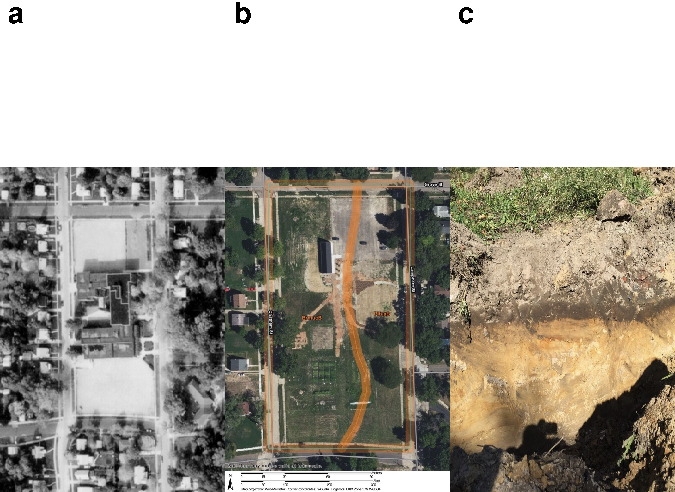
\includegraphics{merge_files/figure-latex/siteFig-1.pdf}
\caption{\label{fig:siteFig}Field site images (a) map © 2022 Wayne State University library digital historical collection showing former school land use from 1981, (b) map data © 2022 USDA-NRCS SSURGO web soil survey showing likely soil class division given field and lab data, (c) soil profile from northeast site area near current education center. Photo credit: (c) Naim Edwards.}
\end{figure}

Site soils can be classified as Technosols (Fig \ref{fig:siteFig}c), given that large metal artifacts can be found throughout various profiles \emph{( FAO (\protect\hyperlink{ref-fao14}{2014}) ; WRB 2015 )}, from when the area was filled in with nearby soils during highway road construction, as was common in mid-western USA industrial manufacturing cities many decades ago in the \emph{1960s} \emph{(\protect\hyperlink{ref-beniston16}{Beniston et al., 2016})}.
Accordingly, the growing area has both a finer- and coarser-textured side (Fig \ref{fig:siteFig}b),
and this study was done on the side with consistent clay of \textasciitilde37\% and a sandy clay loam texture.
Topsoil A horizons are
\textless5 cm
deep, and subsoil B horizons can be \textgreater30.5 cm
deep, with a muted yellow color 10YR 8/4 (Fig \ref{fig:siteFig}c).
A baseline site-level soil lab assessment determined that the top
\emph{10 cm}
of soils around the site together have relatively good organic matter at
\textasciitilde2.5 ±
0.3\%
and nutrient levels, including concentrations of heavy metals like lead and arsenic which were present below harmful government human-contact standards (\url{cfpub.epa.gov/ecotox}).
Site soils were also assesed to have decent but sub-optimal \emph{CO\textsubscript{2}} respiration rates of
0.2 ±
0.04 mg per day
(Table \ref{tab:chemKbl}).
Initial main concerns limiting productivity include high alkaline pH of
8.1 ±
0.1,
lowering availability of existing nutrients, as well as weak aggregate stability of
19 ±
4.4,
leading to concerns with aeration, infiltration, rooting, crusting when dry, and some erosion and runoff, given slopes of \emph{0-4\%} (Table \ref{tab:chemKbl}).

\begin{longtable}[]{@{}ccccc@{}}
\caption{\label{tab:chemKbl}Baseline Soil Health Assessment (Cornell, Ithaca, NY, USA)}\tabularnewline
\toprule()
Kind & Variable & Median (n=10) & Deviation & Descriptor \\
\midrule()
\endfirsthead
\toprule()
Kind & Variable & Median (n=10) & Deviation & Descriptor \\
\midrule()
\endhead
Biological & Organic Matter (\%) & 2.5 & 0.3 & Very Low \\
& Respiration (mg per day) & 0.2 & 0.0 & Medium \\
Physical & Aggregate Stability (\%) & 19.0 & 4.4 & Very Low \\
& Texture (class) & - & - & Fine \\
Chemical & pH & 8.1 & 0.1 & Poor \\
& Phosphorus (ppm) & 2.2 & 1.0 & Medium \\
& Potassium (ppm) & 103.8 & 36.3 & Optimal \\
& Iron (ppm) & 6.0 & 4.4 & Optimal \\
& Magnesium (ppm) & 463.6 & 24.9 & Optimal \\
& Manganese (ppm) & 42.1 & 4.9 & Optimal \\
& Zinc (ppm) & 3.8 & 2.9 & Optimal \\
& Heavy metals (Pb, Al, As, Cu) & - & - & Safe \\
\bottomrule()
\end{longtable}

\hypertarget{design}{%
\subsection{Design}\label{design}}

The study area was a 278 \emph{m\textsuperscript{2}}
section on the East side of the site under the former school building that was divided into 36 separate 4.6 \emph{m\textsuperscript{2}}
plots in nine rows and four columns (Fig \ref{fig:figDesign}a).
Tillage groups spanned the nine columns in adjacent groups of three, while cover crop mix treatments spanned the rows with one row per cover crop mix, totaling 36 plots, or 12 plots per tillage group and nine plots per cover crop mix.
Before applying treatments, approximately 0.2 \emph{m\textsuperscript{3}}
of compost was incorporated into each plot.

\begin{figure}
\centering
\includegraphics{merge_files/figure-latex/designFig-1.pdf}
\caption{\label{fig:designFig}Design images including (a) plot layout and (e) aerial drone view of treated plots after five weeks. Photo credit: (b) Edgar Cardenas.}
\end{figure}

Tillage treatments represented methods of increasing intensity available for small scale agriculture, also varying in cost, machinery needed, and sometimes grower preferences \emph{(\protect\hyperlink{ref-drugova22}{Drugova et al., 2022})}.
Specifially, treatments included no-till with a manual long-tined broadfork \emph{(NT)} tool used for gardens and small farms, roto-tiller \emph{(RT)}, and tractor-till \emph{(TT)} with implements.
Tractor-till plots were worked with a subsoiler, moldboard plow, and roto-tiller implement attached to a tractor \emph{(New Holland 7308)} up to 30.5 cm
deep.
Roto-till plots were treated with a rototiller \emph{(BCS 749)} implement up to 20 cm
deep.
Lastly, no-till plots were worked with only a broadfork up to 10 cm
deep.
All tilling was done once early in the season after one typical compost application and before planting cover crops.

Cover crop mixes were designed primarily based on plants associated with targeted benefits, and as possible, relative simplicity of re-seeding and winter-kill (e.g.~more heat tolerant) \emph{(\protect\hyperlink{ref-clark07}{Clark, 2007})}.
Three mixes were designed to target three functions, with each mix containing three different plant species (Table \ref{tab:crops}).
The mix specifically designed to alleviate compaction generally focused on plants with roots that tend to penetrate and loosen soil well, and ultimately included
crimson clover (\emph{Trifolium incarnatum}),
forage radish (\emph{Raphanus sativus var. longipinnatus}), and
cereal ryegrass (\emph{Secale cereale})
.
The mix targeting weed suppression included heat- and drought-tolerant crops that tend to grow rapidly, allowing them to outcompete other plants--the taxa chosed were
sorghum-sudangrass (\emph{Sorghum bicolor x Sorghum bicolor var. sudanese}),
cowpea/black-eyed pea (\emph{Vigna unguiculata subsp. unguiculata}), and
buckwheat (\emph{Fagopyrum esculentum}).
Lastly, a mix was dedicated to perennial cover crops, which in contrast to annuals can survive the winter and thus tend to accumulate biomass and establish before spring weeds--this mix included
hairy vetch (\emph{Vicia villosa}),
red clover (**), and
wheat (\emph{Triticum aestivum}).
We also had a null control group consisting of established vegetation within the plot, where no additional seeds were sown, so existing plants grew unmanipulated alongside other crop treatments (Fig \ref{fig:figDesign}b).
Cover crops were planted using a manual rolling seeder up to 30 cm between rows and seeds pressed 1-2.5 cm deep varying by cover crop.

\begin{longtable}[]{@{}cc@{}}
\caption{\label{tab:crops}Cover crop mixes}\tabularnewline
\toprule()
Function & Plants \\
\midrule()
\endfirsthead
\toprule()
Function & Plants \\
\midrule()
\endhead
Weed Suppression & Sorghum-Sudangrass \\
& Cowpea/Black-Eyed Pea \\
& Buckwheat \\
Perennial & Hairy Vetch \\
& Red Clover \\
& Wheat \\
Compaction & Forage Radish \\
& Crimson Clover \\
& Cereal Ryegrass \\
Null & Existing vegetation (no manipulation) \\
\bottomrule()
\end{longtable}

\hypertarget{sampling}{%
\subsection{Sampling}\label{sampling}}

Soil compaction-related issues were measured as soil strength (resistance to shear), read as the depth to hardpan layer, or where the soil strength was \textgreater2 MPa
, beyond which roots typically cannot penetrate \emph{(\protect\hyperlink{ref-correa19}{Correa et al., 2019})}.
Soil strength often correlates positively with soil compaction when measured as higher soil density \emph{(\protect\hyperlink{ref-han09}{Han et al., 2009})}, and is also likely in engineered Technosols.
Furthermore, depth to hardpan serves as a measure of potential rooting extent, making it a relevant indicator of common compaction-related issues affecting urban agricultural potential.
Depth to hardpan was measured using a standard 60-degree 1.25 cm wide cone tip penetrometer \emph{(AgraTronix 08180)} in four randomly selected spots within each quarter of every plot.
Readings were recorded to the nearest \emph{2.5 cm (1 inch)} on dry days.

Soil water infiltration down to \emph{10}
cm
depth was measured using a 16.5
wide aluminum cylinder, set away from dense vegetation and any impeding large roots, and recording the time up to 160 sec for \emph{1 L}
to pass through, representing a typical local rainfall onto \textasciitilde0.10 \emph{m\textsuperscript{2}} (\textasciitilde1 \emph{ft\textsuperscript{2}}) of soil area (\url{waterdata.usgs.gov}).

Weed pressure was measured using percent cover, richness, and density, following similar studies \emph{(\protect\hyperlink{ref-storkey18}{Storkey and Neve, 2018})}.
Weed cover was estimated as the total proportion of plot area covered by any weed biomass, descretized into intervals of ten.
Weed richness, a measure of diversity, was recorded by counting the number of unique morphospecies observed in each plot.
Finally, weed density was measured as the number of stems of either of the two most abundant weed taxa, pigweed (\emph{Amaranthus viridis}) and velvetleaf (\emph{Abutilon theophrasti}), also descretized into intervals of ten up to 50 stems per plot.

Five forage radish (Brassica \emph{Raphanus sativus var. longipinnatus}) roots were randomly selected from each plot in the compaction treatment and measured for length, individually, and wet weight, as a cluster.
The length of a radish root was measured from the hypocotyl, or root cap, to where the root became \textasciitilde6.3 mm
wide.

Sampling was done in July and October 2019 and the following Spring.

\hypertarget{statistics}{%
\subsection{Statistics}\label{statistics}}

Field space limited strict plot replication for treatment combinations (\emph{n}=3), and thus inference from advanced nested mixed models \emph{(\protect\hyperlink{ref-silk20}{Silk et al., 2020})}, so analysis focused on specific hypotheses tested using simpler, more conservative non-parametric tests that make few underlying assumptions about data and thus appropriate for data with lower replication.
Kruskal-Wallis tests were run for tillage and cover crop treatments separately, with alpha corrections from 0.05 to 0.01 under multiple comparisons to descriptively parse any treatment interactions, and overall significant treatment effects were followed up by post-hoc Wilcoxon pairwise tests with Holm-corrected p-value adjustments.
All data were centered at plot-level medians, often more robust than means, and where applicable pooled across sampling times given no preliminary significant variation along this axis \emph{(\protect\hyperlink{ref-gomes22}{Gomes, 2022})}, together with minimal relevance to focal hypotheses in field studies
\emph{(\protect\hyperlink{ref-davies15a}{Davies and Gray, 2015})},
and was a general solution to uneven sampling across response variables, also minimally increasing statistical power for hypothesis testing (\emph{n}\textgreater3-6).
For clarity, results figures were designed to reflect statistical models and grouping transparently.
Significant treatment effects were delineated at alpha = 0.05, and marginal significance at 0.05 \textless{} alpha \textless{} 0.1 to align with both convention and decreasing emphasis on strict cutoffs for hypothesis testing \emph{(\protect\hyperlink{ref-curran-everett20}{Curran-Everett, 2020})}.
Treatment effect sizes were estimated with \emph{eta\textsuperscript{2}},
a measure of the proportion of variance in the dependent variable explained by the independent variable using the test statistic and group replication values \emph{(\protect\hyperlink{ref-tomczak14}{Tomczak and Tomczak, 2014})},
and furthermore raw median differences at finer pairwise levels.
All calculations and analyzes were done in R version 4.2.1 (2022-06-23) \emph{(\protect\hyperlink{ref-base}{R Core Team, 2022})} with useful functions from the packages \emph{tidyverse} 1.3.1 \emph{(\protect\hyperlink{ref-tidyverse}{Wickham et al., 2019})}, \emph{rstatix} 0.7.0 and \emph{ggpubr} 0.4.0 \emph{(\protect\hyperlink{ref-rstatix}{Kassambara, 2021})}.
Code stored with Zenodo as \href{https://doi.org/10.5281/zenodo.6800153}{10.5281/zenodo.6800153} \emph{(\protect\hyperlink{ref-softwareMedinaEdwards22}{Medina and Edwards, 2022})} and linked to \url{github.com/nmedina17/must},
documented using R packages
\emph{here} 1.0.1 \emph{(\protect\hyperlink{ref-here}{Müller, 2020})},
\emph{bookdown} 0.27 \emph{(\protect\hyperlink{ref-bookdown2022}{Xie, 2022a})},
\emph{measurements} 1.4.0 \emph{(\protect\hyperlink{ref-measurements}{Birk, 2019})},
\emph{taxize} 0.9.100 \emph{(\protect\hyperlink{ref-taxize2020}{Chamberlain et al., 2020})},
\emph{knitr} 1.39 \emph{(\protect\hyperlink{ref-knitr2022}{Xie, 2022b})}, and
\emph{rmarkdown} 2.14 \emph{(\protect\hyperlink{ref-rmarkdown2022}{Allaire et al., 2022})}
.

\hypertarget{results}{%
\section{Results}\label{results}}

\hypertarget{soil-strength}{%
\subsection{Soil strength}\label{soil-strength}}

Depth to hardpan was affected significantly overall by tillage treatments (
\emph{H} = 38.2,
\emph{df} = 2,
\emph{n} = 72,
\emph{p} = \textless0.0001
) by
\textasciitilde52.4\%
across cover crop treatments (Fig \ref{fig:compactFig}a).
Tractor-till had the largest significant effect on depth to hardpan compared to no-till (
\emph{p\textsubscript{adj}} = \textless0.0001
),
deepening the depth to hardpan by
\textasciitilde9.4 cm (
\textasciitilde83.3\%
) compared to no-till,
down to
\textasciitilde20.6 ±
4.6 cm
across all cover crop mixes.
Roto-till also had a marginally significant effect on depth to hardpan compared to no-till (
\emph{p\textsubscript{adj}} = 0.1
),
deepening the depth to hardpan by
\textasciitilde9.4 cm (
\textasciitilde83.3\%
) compared to no-till, down to
\textasciitilde13.8 ±
1.9 cm
The overall effect from tillage stemmed from significant effects among the perennial (
\emph{p\textsubscript{adj} = \textless0.01}
) and weed suppression (
\emph{p\textsubscript{adj} = \textless0.01}
) mixes (Fig \ref{fig:compactFig}a).
The effect of roto-till was more pronounced in the perennial mix (
\emph{p\textsubscript{adj} = \textless0.01}
), where depth to hardpan was about twice as deep as in no-till plots (Fig \ref{fig:compactFig}a).
There was also a significant difference of
\textasciitilde6.9 cm (
\textasciitilde50\%
) between tractor- and roto-till among all cover crop mixes (Fig \ref{fig:compactFig}a).

\begin{figure}
\centering
\includegraphics{merge_files/figure-latex/compactFig-1.pdf}
\caption{\label{fig:compactFig}Compaction data (a) by tillage, and (b) cover crop mix. Gray dots show plot medians and black point ranges show group mean ± 1 std error and may be small. Significant pairwise post-hoc Wilcoxon test outcomes shown (**** p \textless{} 0.0001, *** p \textless{} 0.001, ** p \textless{} 0.01, * p \textless{} 0.05, *\^{} p \textless{} 0.1, \^{} p \textgreater{} 0.1 or ns)}
\end{figure}

Depth to hardpan was not affected by cover crops among tillage groups overall (
\emph{H} = 2,
\emph{df} = 3,
\emph{n} = 72,
\emph{p} = 0.57
), but was significantly affected by cover crops specifically under no-till conditions (
\emph{p\textsubscript{adj} = \textless0.01}
) (Fig \ref{fig:compactFig}b).
Under no-till, the perennial mix had significantly shallower depth to hardpan compared to both null (
\emph{p\textsubscript{adj} = \textless0.01}
) and weed suppression mixes (
\emph{p\textsubscript{adj} = \textless0.01}
).
Specifically, the perennial mix raised the depth to hardpan by
\textasciitilde2.5 cm (
\textasciitilde16.7\%
) compared to other mixes,
up to
\textasciitilde12.5 ±
7.4 cm
below the soil surface
(Fig \ref{fig:compactFig}b).

\hypertarget{infiltration}{%
\subsection{Infiltration}\label{infiltration}}

Soil infiltration was significantly affected by tillage (
\emph{H} = 8.5,
\emph{df} = 2,
\emph{n} = 48,
\emph{p} = 0.01
) and marginally significantly by cover crop mix (
\emph{H} = 5.9,
\emph{df} = 3,
\emph{n} = 48,
\emph{p} = 0.1
) (Fig \ref{fig:infilFig}).
Roto-till had significantly faster infiltration compared to no-till (
\emph{p\textsubscript{adj}} = 0.027
) and marginally significantly compared to tractor-till (
\emph{p\textsubscript{adj}} = 0.1
), speeding up infiltration by
\textasciitilde14.5\%
compared to each tillage groups,
up to
\textasciitilde{} 13.4 ±
10.7 mL per sec
(Fig \ref{fig:infilFig}a).

\begin{figure}
\centering
\includegraphics{merge_files/figure-latex/infilFig-1.pdf}
\caption{\label{fig:infilFig}Infiltration data (a) by tillage, and (b) cover crop mix. Gray dots show plot medians and black point ranges show group mean ± 1 std error and may be small. Significant pairwise post-hoc Wilcoxon test outcomes shown (**** p \textless{} 0.0001, *** p \textless{} 0.001, ** p \textless{} 0.01, * p \textless{} 0.05, *\^{} p \textless{} 0.1, \^{} p \textgreater{} 0.1)}
\end{figure}

\hypertarget{weed-pressure}{%
\subsection{Weed pressure}\label{weed-pressure}}

Weed density was overall significantly affected by tillage (
\emph{H} = 6.5,
\emph{df} = 2,
\emph{n} = 72,
\emph{p} = 0.039
) by
\textasciitilde25.1\%,
although weed cover (
\emph{H} = 1.6,
\emph{df} = 2,
\emph{n} = 72,
\emph{p} = 0.44
) and richness (
\emph{H} = 0.2,
\emph{df} = 2,
\emph{n} = 36,
\emph{p} = 0.92
) were not
(Fig \ref{fig:weedsFig}a).
Weeds under tractor-till were significantly denser compared to no-till (
\emph{p\textsubscript{adj}} = 0.06
) and marginally significantly compared to roto-till (
\emph{p\textsubscript{adj}} = 0.1
), denser by
\textasciitilde6.5\%
compared to each tillage group,
up to
\textasciitilde{} 8 ±
2 \emph{stems per m\textsuperscript{-2}}
.

\begin{figure}
\centering
\includegraphics{merge_files/figure-latex/weedsFig-1.pdf}
\caption{\label{fig:weedsFig}Weeds data (a) by tillage, and (b) cover crop mix. Gray dots show plot medians and black point ranges show group mean ± 1 std error and may be small. Significant pairwise post-hoc Wilcoxon test outcomes shown (**** p \textless{} 0.0001, *** p \textless{} 0.001, ** p \textless{} 0.01, * p \textless{} 0.05, *\^{} p \textless{} 0.1, \^{} p \textgreater{} 0.1 or ns)}
\end{figure}

All measured weed variables were affected significantly by cover crop mix, including
weed density (
\emph{H} = 20.1,
\emph{df} = 3,
\emph{n} = 72,
\emph{p} = 0.00016
) changing overall by
\textasciitilde6.5\%,
weed cover (
\emph{H} = 31,
\emph{df} = 3,
\emph{n} = 72,
\emph{p} = \textless0.0001
) lowering overall by
\textasciitilde0.5\%
, and
weed richness (
\emph{H} = 10,
\emph{df} = 3,
\emph{n} = 36,
\emph{p} = 0.019
) also lowering overall by
\textasciitilde5.5\%
(Fig \ref{fig:weedsFig}b).
The weed suppression mix had the most detectable effects on both weed density and cover.
The weed suppression mix significantly lowered weed density compared to all other cover crop mix treatments, namely the null (
\emph{p\textsubscript{adj}} = \textless0.001
), perennial (
\emph{p\textsubscript{adj}} = 0.017
), and compaction (
\emph{p\textsubscript{adj}} = 0.025
) mixes, by
\textasciitilde4 \emph{stems m\textsuperscript{-2}} (
\textasciitilde50\%
), down to
\textasciitilde{} 4
\emph{stems per m\textsuperscript{-2}}
.
The weed suppression mix also significantly lowered weed cover compared to all other cover crop mix treatments, namely the null (
\emph{p\textsubscript{adj}} = \textless0.0001
), perennial (
\emph{p\textsubscript{adj}} = \textless0.0001
), and compaction (
\emph{p\textsubscript{adj}} = 0.00093
) mixes, by
\textasciitilde20 \emph{stems m\textsuperscript{-2}} (
\textasciitilde33.3\%
), down to
\textasciitilde{} 40 ±
15\%
.
Finally, the null mix showed significantly higher richness compared to the weed suppression mix (
\emph{p\textsubscript{adj}} = 0.03
) and marginally significantly compared to perennial (
\emph{p\textsubscript{adj}} = 0.1
) and compaction (
\emph{p\textsubscript{adj}} = 0.2
) mixes,
up to
\textasciitilde{} 4
taxa.

\hypertarget{yield}{%
\subsection{Yield}\label{yield}}

Radish yield was not significantly affected by tillage (
\emph{H} = 1.4,
\emph{df} = 2,
\emph{n} = 8,
\emph{p} = 0.5
), and centered at
\textasciitilde{} 67.8
\emph{g m\textsuperscript{-2}}
--\textgreater{}
and
\textasciitilde{} 13.2 cm
--\textgreater{}
--\textgreater{}
long (Fig \ref{fig:yieldFig}).
Notably, radish yield under roto-till tended to be lower compared to other treatments, and also appeared more variable in mass.

\begin{figure}
\centering
\includegraphics{merge_files/figure-latex/yieldFig-1.pdf}
\caption{\label{fig:yieldFig}Yield data (a) from no-till, (b) tractor-till, and (c) all tillage groups. Gray dots show plot medians and black point ranges show group mean ± 1 std error and may be small. Photo credits: Naim Edwards.}
\end{figure}

\hypertarget{discussion}{%
\section{Discussion}\label{discussion}}

Overall, this study informs urban soil management by supporting the use of tillage to address compaction-related issues and improve infiltration, together with the use of cover crops to reduce weed pressure.
We hypothesized that cover crop use would be comparable to tillage effects, which was in part supported, because overall tillage significantly deepened the depth to hardpan by \textasciitilde0.5
cm
(Fig \ref{fig:compactFig}a), which was within the range of effect sizes measured among the various cover crop mixes within the no-till treatment (Fig \ref{fig:compactFig}b).
It was notable that native vegetation under no-till also showed the deepest depth to hardpan, in part supporting a fallow approach instead of cover crops, but using cover crops may have additional benefits like improving nutrient retention \emph{(\protect\hyperlink{ref-tonitto06}{Tonitto et al., 2006})}.
Additionally, infiltration was significantly affected by tillage, with roto-till showing the fastest rates (Fig \ref{fig:infilFig}a), which agreed with our predictions.
Furthermore, weed pressure was significantly affected by both cover crop mixes and tillage (Fig \ref{fig:weedsFig}); although effects from cover crop mixes, especially the weed suppression mix, were more widespread among multiple measured variables (Fig \ref{fig:weedsFig}b).
Despite these significant effects on soils, infiltration, and weeds, yields did not respond to tillage treatments in this study.

Short-term soil compaction and soil strength issues are commonly alleviated by annual tilling \emph{(\protect\hyperlink{ref-badalikova10}{Badalíková, 2010}; \protect\hyperlink{ref-salem15}{Salem et al., 2015})}, and in addition to validating this practice, this study showed that cover cropping can also be used to manage soil strength under no-till, although effects vary by mixture of taxa used.
Under tillage, this study validates that tillage method intensity corresponds negatively with depth to hardpan.
This can be due to changes in either soil density or remnant moisture at depth, but given that infiltration results did not mirror soil strength results, it may be more likely that changes to soil density, either from textural or structural (arrangement) changes, are the larger underlying cause compared to consistent soil moisture differences.
This study additionally clarifies that tractor-till can lower soil strength in slightly deeper soils below main root zones under
\textasciitilde20.6 ±
4.6 cm
as well as suggests that roto-till can be useful under perennial crops.
Although under annuals, no-till can be just as effective as roto-till, saving grower time, energy, and cost for areas with crops harvested before rooting surpasses \emph{\textasciitilde10 cm}
\emph{(\protect\hyperlink{ref-krause95}{Krause and Black, 1995})}.
It was notable that under tractor-till, the soil hardpan was detected at a shallower depth than that where the initial treatment was done, suggesting short-term particle resettlement, which may occur following the redistribution and separation of macroaggregates into microaggregate fractions \emph{(\protect\hyperlink{ref-zheng18}{Zheng et al., 2018})}.
For urban Technosol soils, it is worth noting that some initial tillage may help remove large metal artifacts and legacy construction debris -- such as rebar, wires, cables, bricks, cinder blocks, and pipes -- that could limit root growth under stricter no-till management.
Additionally, results suggest that when used together, tillage may obscure varying but notable effects of cover crops on compaction, however, cover crops would still provide separate benefits to soils, like available macro-nutrients \emph{(\protect\hyperlink{ref-chapagain20}{Chapagain et al., 2020})}.
Under no-till, this study found that perennial crop mixes can have significant effects on soil strength, but rather than deep roots loosening soils, in some cases depth to hardpan can instead become shallower.
This shallower depth to hardpan may be due to dense root mats that can form under grasses \emph{(\protect\hyperlink{ref-douglas92}{Douglas et al., 1992})}, such as sorghum-sudangrass, which could collectively act as a barrier to water flow, especially in otherwise dense soils, helping water to pool under the soil surface \emph{(\protect\hyperlink{ref-hoogmoed80}{Hoogmoed and Bouma, 1980})}.
Other studies have generally found similar results that suggest short-term benefits of tillage to soil functions, while acknowledging tradeoffs with long-term costs of tillage \emph{(\protect\hyperlink{ref-ozpinar06}{Ozpinar and Cay, 2006})}.

Water infiltration is a key function of wide interest for urban environmental management, needed to not only increase available root water but also to reduce erosion and potentially contaminated storm-water runoff and flooding \emph{(\protect\hyperlink{ref-masoner19}{Masoner et al., 2019})} after even short heavy rains, due to soil sealing by concrete near hillslopes \emph{(\protect\hyperlink{ref-dreelin06}{Dreelin et al., 2006})}.
This study found that roto-till resulted in significantly faster infiltration compared to no-till, unlike tractor-till, suggesting that roto-till management can generally be effective for improving infiltration and drainage.
This result could be explained by medium intensity roto-till increasing soil macro-porosity, which compared to micro-pores bind water less tightly, allowing soil water to flow faster \emph{(\protect\hyperlink{ref-gerke06}{Gerke, 2006})}.
In contrast, the tractor diffused tillage energy across deeper soil volume, lowering the density of any added soil macro-pores and thereby making it easier for soil particles to settle back together, whereas no-till may have needed more time to improve macro-porosity via organic matter effects on soil structure \emph{(\protect\hyperlink{ref-king20}{King, 2020})}.
It is also possible that this result could be explained by compost incorporation, where tractor-till incorporated the same amount of compost more diffusely throughout the soil profile, and thereby diluting potential benefits of compost on water infiltration, such as by improving seasonal soil aggregation \emph{(\protect\hyperlink{ref-bach19}{\textbf{bach19?}})}.

In urban settings, weed suppression not only alleviates competition with crops that may already be stressed, but also lowers human health risks, including asthma and other respiratory issues stemming from allergens like pollen \emph{(\protect\hyperlink{ref-katz14}{Katz and Carey, 2014})}, and this study shows evidence that cover crops may be better at weed suppression than tilling \emph{(\protect\hyperlink{ref-barberi01}{Bàrberi and Lo Cascio, 2001}; \protect\hyperlink{ref-cordeau20}{Cordeau et al., 2020})}.
Tractor-till lowered soil strength to the deepest hardpan layer at the cost of showing the highest density of the two most common weeds, velvet leaf (\emph{Abutilon theophrasti}) and pigweed (\emph{Palmer amaranth}).
This may have been due to their fast-growing weed life histories, which can allow them to grow denser root systems in more porous soils, despite experiencing variable soil microbiomes nearby \emph{(\protect\hyperlink{ref-korneykova21}{Korneykova et al., 2021})}, possibly helping explain slower infiltration, with roots that could re-sprout more, clonally and/or from seed banks \emph{(\protect\hyperlink{ref-hesse07}{Hesse et al., 2007})}.
Most notably for weed suppression, the targeted mix consisting of sorghum-sudangrass, buckwheat, and cowpea indeed significantly reduced both weed density and richness by about half compared to the other cover crop mixes.
This result agrees with other studies pairing buckwheat and sorghum-sudangrass \emph{(\protect\hyperlink{ref-smith15}{Smith et al., 2015})}, and may have occurred due to any of several reasons:
competitive exclusion of other weeds by either taxon, such via allelopathic chemical root defenses \emph{(\protect\hyperlink{ref-weston89}{Weston et al., 1989})};
competition for light \emph{(\protect\hyperlink{ref-liu09b}{Liu et al., 2009})};
better phosphorus mining and use by buckwheat \emph{(\protect\hyperlink{ref-zhu02}{Zhu et al., 2002})};
facilitation or amplification of these listed effects by cowpea's added nitrogen supply \emph{(\protect\hyperlink{ref-martins03}{Martins et al., 2003}; \protect\hyperlink{ref-sanginga00}{Sanginga et al., 2000})};
and/or existing adaptations to poor dry soils \emph{(\protect\hyperlink{ref-barberi18}{Bàrberi et al., 2018})} allowing high biomass accumulation.
Given both effectiveness and relative ease of re-seeding and winter-kill, this weed suppression mix could serve well to frame crop beds, keep out encroaching weeds, or reduce weed pressure in an area that might be planted in the fall or following season.

Despite overall significant effects by tillage on soil strength, infiltration, and weeds, tillage did not significantly affect radish yield, which in fact agrees with other similar studies, in contrast to common hypotheses.
In this study radish yield appeared to be lower and more variable under roto-till, which could be explained in part by the leaching of otherwise available nutrients due to observed faster infiltration under roto-till.
Furthermore, as is this study does not rule out more complex relationships between soil strength, infiltration, and crop yield, as suggested by emerging ideas \emph{(\protect\hyperlink{ref-ryan07}{Ryan et al., 2007}; \protect\hyperlink{ref-vandermeer17}{Vandermeer and Perfecto, 2017})}.
With further replication, future similar studies no-till might be expected to show slightly higher yields \emph{(\protect\hyperlink{ref-nunes18}{Nunes et al., 2018})}, due to resulting longer-term reservoirs of water and nutrients, like from mulched compost, less reliance on transient influxes from infiltration \emph{(\protect\hyperlink{ref-schlegel15}{Schlegel et al., 2015}; \protect\hyperlink{ref-schlegel95}{Schlegel and Havlin, 1995})}, and better soil structure \emph{(\protect\hyperlink{ref-du15}{Du et al., 2015}; \protect\hyperlink{ref-sheehy15}{Sheehy et al., 2015})}.
However, despite these reasonable hypotheses, recent studies appear to converge with results shown here, namely that benefits to soil from no-till may not scale up to detectably affect yields \emph{(\protect\hyperlink{ref-martinez16}{Martínez et al., 2016}; \protect\hyperlink{ref-pittelkow15}{Pittelkow et al., 2015}; \protect\hyperlink{ref-vandenbygaart16}{VandenBygaart, 2016})}.
While forage radish itself may not respond to management, it may still confer benefits to surrounding soils, eventually lowering soil strength and building soil structure, such as with minimal or no mechanical tillage \emph{(\protect\hyperlink{ref-chen10b}{Chen and Weil, 2010}; \protect\hyperlink{ref-lawley11}{Lawley et al., 2011})}.
Together with others, this study suggests a need for future studies to tie yield to land management strategies, including in urban clay soils, to aid small-scale growers in addressing legacy compaction and pH issues, potentially acknolwedging short-term benefits of occassional tillage \emph{(\protect\hyperlink{ref-blanco-canqui20}{Blanco-Canqui and Wortmann, 2020}; \protect\hyperlink{ref-ekboir01}{Ekboir, 2001})}.

Taken together, this study presents findings that, in addition to validating previous studies supporting general tillage for short-term soil fertility, also supports the targeted use of medium-intensity roto-till and cover crop mixtures \emph{(\protect\hyperlink{ref-chapagain20}{Chapagain et al., 2020})} specifically for weed suppression.
Overall, this study supported the use of roto-till, but not no-till or tractor-till, against a one inch rain event, since both others showed rates of only
\textasciitilde{} 6.2 ±
mL per sec
which would likely be associated with more rain water runoff and soil erosion, worse field drainage, and pooling or flooding into roads.
Regarding cover crops, this study suggests that cover crop mixes can generally affect infiltration, though specifically perennials may not have notable significant effects on infiltration rates, despite detectable effects on soil strength.
Based on these findings, roto-till (alongside compost) can be and effective practice to specifically improve urban soil water infiltration, at least in the short-term, after which no-till may prevail \emph{(\protect\hyperlink{ref-cusser20}{Cusser et al., 2020})}.
This study serves as a model demonstration of both widely-accessible and effective strategies for growing on re-purposed urban soils after industrial land-use turnover.
Overall, we advocate for the maximal use of cover crop mixes for various target functions, with medium-intensity tillage to jump-start urban cultivation.

\newpage

\hypertarget{funding}{%
\section*{Funding}\label{funding}}
\addcontentsline{toc}{section}{Funding}

\emph{This research did not receive any specific grant from funding agencies in the public, commercial, or not-for-profit sectors.}

\hypertarget{declaration-of-interests}{%
\section*{Declaration of interests}\label{declaration-of-interests}}
\addcontentsline{toc}{section}{Declaration of interests}

Authors declare no conflicts of interest.

\hypertarget{acknowledgements}{%
\section*{Acknowledgements}\label{acknowledgements}}
\addcontentsline{toc}{section}{Acknowledgements}

Authors thank Brother Nature Produce, Earthworks Urban Farm, and Georgia Street Community Collective for early project input; site intern JH for field assistance; volunteer GV for site background help; and previous anonymous reviewers and peers KS, ZHF, and JK for discussion of initial drafts.

\hypertarget{author-contributions}{%
\section*{Author contributions}\label{author-contributions}}
\addcontentsline{toc}{section}{Author contributions}

NE conceived, designed, and performed the study; NE and NM helped collect data; NM analyzed data; NE wrote the initial report. All authors wrote and revised second draft; NM wrote the third draft; all authors approved recent version.

\hypertarget{data-statement}{%
\section*{Data statement}\label{data-statement}}
\addcontentsline{toc}{section}{Data statement}

Code stored with Zenodo as \href{https://doi.org/10.5281/zenodo.6800153}{10.5281/zenodo.6800153} \emph{(\protect\hyperlink{ref-softwareMedinaEdwards22}{Medina and Edwards, 2022})} and linked to \url{github.com/nmedina17/must}.

\newpage

\hypertarget{references}{%
\section*{References}\label{references}}
\addcontentsline{toc}{section}{References}

\hypertarget{refs}{}
\begin{CSLReferences}{1}{0}
\leavevmode\vadjust pre{\hypertarget{ref-acuto18}{}}%
Acuto, M., Parnell, S., Seto, K.C., 2018. Building a global urban science. Nature Sustainability 1, 2--4. \url{https://doi.org/10.1038/s41893-017-0013-9}

\leavevmode\vadjust pre{\hypertarget{ref-rmarkdown2022}{}}%
Allaire, J., Xie, Y., McPherson, J., Luraschi, J., Ushey, K., Atkins, A., Wickham, H., Cheng, J., Chang, W., Iannone, R., 2022. \href{https://github.com/rstudio/rmarkdown}{Rmarkdown: Dynamic documents for r}.

\leavevmode\vadjust pre{\hypertarget{ref-amundson15}{}}%
Amundson, R., Berhe, A.A., Hopmans, J.W., Olson, C., Sztein, A.E., Sparks, D.L., 2015. Soil science. {Soil} and human security in the 21st century. Science (New York, N.Y.) 348, 1261071. \url{https://doi.org/10.1126/science.1261071}

\leavevmode\vadjust pre{\hypertarget{ref-anderson07}{}}%
Anderson, R.L., 2007. Managing weeds with a dualistic approach of prevention and control. {A} review. Agronomy for Sustainable Development 27, 13--18. \url{https://doi.org/10.1051/agro:2006027}

\leavevmode\vadjust pre{\hypertarget{ref-badalikova10}{}}%
Badalíková, B., 2010. Influence of {Soil Tillage} on {Soil Compaction}, in: Dedousis, A.P., Bartzanas, T. (Eds.), Soil {Engineering}. {Springer Berlin Heidelberg}, {Berlin, Heidelberg}, pp. 19--30. \url{https://doi.org/10.1007/978-3-642-03681-1_2}

\leavevmode\vadjust pre{\hypertarget{ref-baraibar20}{}}%
Baraibar, B., Murrell, E.G., Bradley, B.A., Barbercheck, M.E., Mortensen, D.A., Kaye, J.P., White, C.M., 2020. Cover crop mixture expression is influenced by nitrogen availability and growing degree days. PLOS ONE 15, e0235868. \url{https://doi.org/10.1371/journal.pone.0235868}

\leavevmode\vadjust pre{\hypertarget{ref-barberi18}{}}%
Bàrberi, P., Bocci, G., Carlesi, S., Armengot, L., Blanco-Moreno, J.M., Sans, F.X., 2018. Linking species traits to agroecosystem services: A functional analysis of weed communities. Weed Research 58, 76--88. \url{https://doi.org/10.1111/wre.12283}

\leavevmode\vadjust pre{\hypertarget{ref-barberi01}{}}%
Bàrberi, P., Lo Cascio, B., 2001. Long-term tillage and crop rotation effects on weed seedbank size and composition. Weed Research 41, 325--340. \url{https://doi.org/10.1046/j.1365-3180.2001.00241.x}

\leavevmode\vadjust pre{\hypertarget{ref-bazzoffi98}{}}%
Bazzoffi, P., 1998. The effect of urban refuse compost and different tractors tyres on soil physical properties, soil erosion and maize yield. Soil and Tillage Research 48, 275--286. \url{https://doi.org/10.1016/S0167-1987(98)00133-0}

\leavevmode\vadjust pre{\hypertarget{ref-bedoussac15}{}}%
Bedoussac, L., Journet, E.-P., Hauggaard-Nielsen, H., Naudin, C., Corre-Hellou, G., Jensen, E.S., Prieur, L., Justes, E., 2015. Ecological principles underlying the increase of productivity achieved by cereal-grain legume intercrops in organic farming. {A} review. Agronomy for Sustainable Development 35, 911--935. \url{https://doi.org/10.1007/s13593-014-0277-7}

\leavevmode\vadjust pre{\hypertarget{ref-beniston16}{}}%
Beniston, J.W., Lal, R., Mercer, K.L., 2016. Assessing and {Managing Soil Quality} for {Urban Agriculture} in a {Degraded Vacant Lot Soil}: {ASSESSING AND MANAGING SOIL QUALITY FOR URBAN AGRICULTURE}. Land Degradation \& Development 27, 996--1006. \url{https://doi.org/10.1002/ldr.2342}

\leavevmode\vadjust pre{\hypertarget{ref-measurements}{}}%
Birk, M.A., 2019. \href{https://CRAN.R-project.org/package=measurements}{Measurements: Tools for units of measurement}.

\leavevmode\vadjust pre{\hypertarget{ref-blanco-canqui20}{}}%
Blanco-Canqui, H., Wortmann, C.S., 2020. Does occasional tillage undo the ecosystem services gained with no-till? {A} review. Soil and Tillage Research 198, 104534. \url{https://doi.org/10.1016/j.still.2019.104534}

\leavevmode\vadjust pre{\hypertarget{ref-blesh17}{}}%
Blesh, J., 2017. Functional traits in cover crop mixtures: {Biological} nitrogen fixation and multifunctionality. Journal of Applied Ecology 55, 38--48. \url{https://doi.org/10.1111/1365-2664.13011}

\leavevmode\vadjust pre{\hypertarget{ref-block12}{}}%
Block, D.R., Chávez, N., Allen, E., Ramirez, D., 2012. Food sovereignty, urban food access, and food activism: Contemplating the connections through examples from {Chicago}. Agriculture and Human Values 29, 203--215. \url{https://doi.org/10.1007/s10460-011-9336-8}

\leavevmode\vadjust pre{\hypertarget{ref-bourke21}{}}%
Bourke, P.M., Evers, J.B., Bijma, P., van Apeldoorn, D.F., Smulders, M.J.M., Kuyper, T.W., Mommer, L., Bonnema, G., 2021. Breeding {Beyond Monoculture}: {Putting} the {``{Intercrop}''} {Into Crops}. Frontiers in Plant Science 12, 734167. \url{https://doi.org/10.3389/fpls.2021.734167}

\leavevmode\vadjust pre{\hypertarget{ref-cambou18}{}}%
Cambou, A., Shaw, R.K., Huot, H., Vidal-Beaudet, L., Hunault, G., Cannavo, P., Nold, F., Schwartz, C., 2018. Estimation of soil organic carbon stocks of two cities, {New York City} and {Paris}. Science of The Total Environment 644, 452--464. \url{https://doi.org/10.1016/j.scitotenv.2018.06.322}

\leavevmode\vadjust pre{\hypertarget{ref-catania18}{}}%
Catania, P., Badalucco, L., Laudicina, V.A., Vallone, M., 2018. Effects of tilling methods on soil penetration resistance, organic carbon and water stable aggregates in a vineyard of semiarid {Mediterranean} environment. Environmental Earth Sciences 77, 348. \url{https://doi.org/10.1007/s12665-018-7520-5}

\leavevmode\vadjust pre{\hypertarget{ref-taxize2020}{}}%
Chamberlain, S., Szoecs, E., Foster, Z., Arendsee, Z., Boettiger, C., Ram, K., Bartomeus, I., Baumgartner, J., O'Donnell, J., Oksanen, J., Tzovaras, B.G., Marchand, P., Tran, V., Salmon, M., Li, G., Grenié, M., 2020. \href{https://github.com/ropensci/taxize}{Taxize: Taxonomic information from around the web}.

\leavevmode\vadjust pre{\hypertarget{ref-chapagain20}{}}%
Chapagain, T., Lee, E.A., Raizada, M.N., 2020. The {Potential} of {Multi-Species Mixtures} to {Diversify Cover Crop Benefits}. Sustainability 12, 2058. \url{https://doi.org/10.3390/su12052058}

\leavevmode\vadjust pre{\hypertarget{ref-chen10b}{}}%
Chen, G., Weil, R.R., 2010. Penetration of cover crop roots through compacted soils. Plant and Soil 331, 31--43. \url{https://doi.org/10.1007/s11104-009-0223-7}

\leavevmode\vadjust pre{\hypertarget{ref-clark07}{}}%
Clark, A. (Ed.), 2007. Managing cover crops profitably, 3rd ed. ed, Handbook series. {Sustainable Agriculture Research \& Education (SARE)}, {College Park, MD}.

\leavevmode\vadjust pre{\hypertarget{ref-clendenning16}{}}%
Clendenning, J., Dressler, W.H., Richards, C., 2016. Food justice or food sovereignty? {Understanding} the rise of urban food movements in the {USA}. Agriculture and Human Values 33, 165--177. \url{https://doi.org/10.1007/s10460-015-9625-8}

\leavevmode\vadjust pre{\hypertarget{ref-cogger05}{}}%
Cogger, C.G., 2005. Potential {Compost Benefits} for {Restoration Of Soils Disturbed} by {Urban Development}. Compost Science \& Utilization 13, 243--251. \url{https://doi.org/10.1080/1065657X.2005.10702248}

\leavevmode\vadjust pre{\hypertarget{ref-cordeau20}{}}%
Cordeau, S., Baudron, A., Adeux, G., 2020. Is {Tillage} a {Suitable Option} for {Weed Management} in {Conservation Agriculture}? Agronomy 10, 1746. \url{https://doi.org/10.3390/agronomy10111746}

\leavevmode\vadjust pre{\hypertarget{ref-correa19}{}}%
Correa, J., Postma, J.A., Watt, M., Wojciechowski, T., 2019. Soil compaction and the architectural plasticity of root systems. Journal of Experimental Botany 70, 6019--6034. \url{https://doi.org/10.1093/jxb/erz383}

\leavevmode\vadjust pre{\hypertarget{ref-curran-everett20}{}}%
Curran-Everett, D., 2020. Evolution in statistics: {\emph{P}} values, statistical significance, kayaks, and walking trees. Advances in Physiology Education 44, 221--224. \url{https://doi.org/10.1152/advan.00054.2020}

\leavevmode\vadjust pre{\hypertarget{ref-cusser20}{}}%
Cusser, S., Bahlai, C., Swinton, S.M., Robertson, G.P., Haddad, N.M., 2020. Long-term research avoids spurious and misleading trends in sustainability attributes of no-till. Global Change Biology 26, 3715--3725. \url{https://doi.org/10.1111/gcb.15080}

\leavevmode\vadjust pre{\hypertarget{ref-daftary-steel15}{}}%
Daftary-Steel, S., Herrera, H., Porter, C., 2015. The {Unattainable Trifecta} of {Urban Agriculture}. Journal of Agriculture, Food Systems, and Community Development 19--32. \url{https://doi.org/10.5304/jafscd.2015.061.014}

\leavevmode\vadjust pre{\hypertarget{ref-daniel07}{}}%
Daniel, P., 2007. African {American Farmers} and {Civil Rights} 37.

\leavevmode\vadjust pre{\hypertarget{ref-davies15a}{}}%
Davies, G.M., Gray, A., 2015. Don't let spurious accusations of pseudoreplication limit our ability to learn from natural experiments (and other messy kinds of ecological monitoring). Ecology and Evolution 5, 5295--5304. \url{https://doi.org/10.1002/ece3.1782}

\leavevmode\vadjust pre{\hypertarget{ref-decarcer19}{}}%
de Cárcer, P.S., Sinaj, S., Santonja, M., Fossati, D., Jeangros, B., 2019. Long-term effects of crop succession, soil tillage and climate on wheat yield and soil properties. Soil and Tillage Research 190, 209--219. \url{https://doi.org/10.1016/j.still.2019.01.012}

\leavevmode\vadjust pre{\hypertarget{ref-deeb19}{}}%
Deeb, M., Groffman, P.M., Blouin, M., Egendorf, S.P., Vergnes, A., Vasenev, V., Cao, D.L., Walsh, D., Morin, T., Séré, G., 2019. Constructed {Technosols} are key to the sustainable development of urban green infrastructure. \url{https://doi.org/10.5194/soil-2019-85}

\leavevmode\vadjust pre{\hypertarget{ref-douglas92}{}}%
Douglas, J.T., Koppi, A.J., Moran, C.J., 1992. Alteration of the structural attributes of a compact clay loam soil by growth of a perennial grass crop. Plant and Soil 139, 195--202. \url{https://doi.org/10.1007/BF00009310}

\leavevmode\vadjust pre{\hypertarget{ref-dreelin06}{}}%
Dreelin, E.A., Fowler, L., Ronald Carroll, C., 2006. A test of porous pavement effectiveness on clay soils during natural storm events. Water Research 40, 799--805. \url{https://doi.org/10.1016/j.watres.2005.12.002}

\leavevmode\vadjust pre{\hypertarget{ref-drugova22}{}}%
Drugova, T., Curtis, K.R., Ward, R.A., 2022. Producer preferences for drought management strategies in the arid west. Renewable Agriculture and Food Systems 37, 14--23. \url{https://doi.org/10.1017/S1742170521000259}

\leavevmode\vadjust pre{\hypertarget{ref-du15}{}}%
Du, Z., Ren, T., Hu, C., Zhang, Q., 2015. Transition from intensive tillage to no-till enhances carbon sequestration in microaggregates of surface soil in the {North China Plain}. Soil and Tillage Research 146, 26--31. \url{https://doi.org/10.1016/j.still.2014.08.012}

\leavevmode\vadjust pre{\hypertarget{ref-edwards16}{}}%
Edwards, N., 2016. Effects of {Garden Attributes} on {Ant} ( {Formicidae} ) {Species Richness} and {Potential} for {Pest Control}. Urban Agriculture \& Regional Food Systems 1--11. \url{https://doi.org/10.2134/urbanag2015.01.1405}

\leavevmode\vadjust pre{\hypertarget{ref-ekboir01}{}}%
Ekboir, J., 2001. Developing {No-Till Packages} for {Small-Scale Farmers}.

\leavevmode\vadjust pre{\hypertarget{ref-fao14}{}}%
FAO, 2014. World reference base for soil resources 2014: International soil classification system for naming soils and creating legends for soil maps. {FAO}, {Rome}.

\leavevmode\vadjust pre{\hypertarget{ref-garbach17}{}}%
Garbach, K., Milder, J.C., DeClerck, F.A.J., Montenegro de Wit, M., Driscoll, L., Gemmill-Herren, B., 2017. Examining multi-functionality for crop yield and ecosystem services in five systems of agroecological intensification. International Journal of Agricultural Sustainability 15, 11--28. \url{https://doi.org/10.1080/14735903.2016.1174810}

\leavevmode\vadjust pre{\hypertarget{ref-garcia-gonzalez18}{}}%
García-González, I., Hontoria, C., Gabriel, J.L., Alonso-Ayuso, M., Quemada, M., 2018. Cover crops to mitigate soil degradation and enhance soil functionality in irrigated land. Geoderma 322, 81--88. \url{https://doi.org/10.1016/j.geoderma.2018.02.024}

\leavevmode\vadjust pre{\hypertarget{ref-garcia-sempere19}{}}%
García-Sempere, A., Morales, H., Hidalgo, M., Ferguson, B.G., Rosset, P., Nazar-Beutelspacher, A., 2019. Food {Sovereignty} in the city?: {A} methodological proposal for evaluating food sovereignty in urban settings. Agroecology and Sustainable Food Systems 43, 1145--1173. \url{https://doi.org/10.1080/21683565.2019.1578719}

\leavevmode\vadjust pre{\hypertarget{ref-gerke06}{}}%
Gerke, H.H., 2006. Preferential flow descriptions for structured soils. Journal of Plant Nutrition and Soil Science 169, 382--400. \url{https://doi.org/10.1002/jpln.200521955}

\leavevmode\vadjust pre{\hypertarget{ref-gomes22}{}}%
Gomes, D.G.E., 2022. Should {I} use fixed effects or random effects when {I} have fewer than five levels of a grouping factor in a mixed-effects model? PeerJ 10, e12794. \url{https://doi.org/10.7717/peerj.12794}

\leavevmode\vadjust pre{\hypertarget{ref-grossman03}{}}%
Grossman, J.M., 2003. Exploring farmer knowledge of soil processes in organic coffee systems of {Chiapas}, {Mexico}. Geoderma 111, 267--287. \url{https://doi.org/10.1016/S0016-7061(02)00268-9}

\leavevmode\vadjust pre{\hypertarget{ref-grossman05}{}}%
Grossman, J.M., Sheaffer, C., Wyse, D., Graham, P.H., 2005. Characterization of slow-growing root nodule bacteria from {Inga} oerstediana in organic coffee agroecosystems in {Chiapas}, {Mexico}. Applied Soil Ecology 29, 236--251. \url{https://doi.org/10.1016/j.apsoil.2004.12.008}

\leavevmode\vadjust pre{\hypertarget{ref-han09}{}}%
Han, S.-K., Han, H.-S., Page-Dumroese, D.S., Johnson, L.R., 2009. Soil compaction associated with cut-to-length and whole-tree harvesting of a coniferous forest. Canadian Journal of Forest Research 39, 976--989. \url{https://doi.org/10.1139/X09-027}

\leavevmode\vadjust pre{\hypertarget{ref-hesse07}{}}%
Hesse, E., Rees, M., Müller-Schärer, H., 2007. Seed bank persistence of clonal weeds in contrasting habitats: Implications for control. Plant Ecology 190, 233--243. \url{https://doi.org/10.1007/s11258-006-9203-7}

\leavevmode\vadjust pre{\hypertarget{ref-hill85}{}}%
Hill, R.L., Horton, R., Cruse, R.M., 1985. Tillage {Effects} on {Soil Water Retention} and {Pore Size Distribution} of {Two Mollisols}. Soil Science Society of America Journal 49, 1264--1270. \url{https://doi.org/10.2136/sssaj1985.03615995004900050039x}

\leavevmode\vadjust pre{\hypertarget{ref-hoogmoed80}{}}%
Hoogmoed, W.B., Bouma, J., 1980. A {Simulation Model} for {Predicting Infiltration} into {Cracked Clay Soil}. Soil Science Society of America Journal 44, 458--461. \url{https://doi.org/10.2136/sssaj1980.03615995004400030003x}

\leavevmode\vadjust pre{\hypertarget{ref-rstatix}{}}%
Kassambara, A., 2021. \href{https://CRAN.R-project.org/package=rstatix}{Rstatix: Pipe-friendly framework for basic statistical tests}.

\leavevmode\vadjust pre{\hypertarget{ref-katz14}{}}%
Katz, D.S.W., Carey, T.S., 2014. Heterogeneity in ragweed pollen exposure is determined by plant composition at small spatial scales. Science of the Total Environment 485--486, 435--440. \url{https://doi.org/10.1016/j.scitotenv.2014.03.099}

\leavevmode\vadjust pre{\hypertarget{ref-king20}{}}%
King, A.E., 2020. Soil {Organic Matter} as {Catalyst} of {Crop Resource Capture}. Frontiers in Environmental Science 8, 8.

\leavevmode\vadjust pre{\hypertarget{ref-korneykova21}{}}%
Korneykova, M.V., Vasenev, V.I., Nikitin, D.A., Soshina, A.S., Dolgikh, A.V., Sotnikova, Y.L., 2021. Urbanization {Affects Soil Microbiome Profile Distribution} in the {Russian Arctic Region}. International Journal of Environmental Research and Public Health 18, 11665. \url{https://doi.org/10.3390/ijerph182111665}

\leavevmode\vadjust pre{\hypertarget{ref-krause95}{}}%
Krause, M.A., Black, J.R., 1995. Optimal {Adoption Strategies} for {No-till Technology} in {Michigan}. Review of Agricultural Economics 17, 299. \url{https://doi.org/10.2307/1349575}

\leavevmode\vadjust pre{\hypertarget{ref-kumar16}{}}%
Kumar, K., Hundal, L.S., 2016. Soil in the {City}: {Sustainably Improving Urban Soils}. Journal of Environmental Quality 45, 2--8. \url{https://doi.org/10.2134/jeq2015.11.0589}

\leavevmode\vadjust pre{\hypertarget{ref-kuzyakov19}{}}%
Kuzyakov, Y., Zamanian, K., 2019. Reviews and syntheses: {Agropedogenesis} \textendash{} humankind as the sixth soil-forming factor and attractors of agricultural soil degradation. Biogeosciences 16, 4783--4803. \url{https://doi.org/10.5194/bg-16-4783-2019}

\leavevmode\vadjust pre{\hypertarget{ref-lal07}{}}%
Lal, R., 2007. Soil {Science} and the {Carbon Civilization} 71, 1425--1437. \url{https://doi.org/10.2136/sssaj2007.0001}

\leavevmode\vadjust pre{\hypertarget{ref-lal15}{}}%
Lal, R., Negassa, W., Lorenz, K., 2015. Carbon sequestration in soil. Current Opinion in Environmental Sustainability 15, 79--86. \url{https://doi.org/10.1016/j.cosust.2015.09.002}

\leavevmode\vadjust pre{\hypertarget{ref-lawley11}{}}%
Lawley, Y.E., Weil, R.R., Teasdale, J.R., 2011. Forage {Radish Cover Crop Suppresses Winter Annual Weeds} in {Fall} and {Before Corn Planting}. Agronomy Journal 103, 137--144. \url{https://doi.org/10.2134/agronj2010.0187}

\leavevmode\vadjust pre{\hypertarget{ref-liu09b}{}}%
Liu, J.G., Mahoney, K.J., Sikkema, P.H., Swanton, C.J., 2009. The importance of light quality in crop-weed competition: {Light} quality and crop competition. Weed Research 49, 217--224. \url{https://doi.org/10.1111/j.1365-3180.2008.00687.x}

\leavevmode\vadjust pre{\hypertarget{ref-london21}{}}%
London, J.K., Cutts, B.B., Schwarz, K., Schmidt, L., Cadenasso, M.L., 2021. Unearthing the entangled roots of urban agriculture. Agriculture and Human Values 38, 205--220. \url{https://doi.org/10.1007/s10460-020-10158-x}

\leavevmode\vadjust pre{\hypertarget{ref-martinez16}{}}%
Martínez, I., Chervet, A., Weisskopf, P., Sturny, W.G., Etana, A., Stettler, M., Forkman, J., Keller, T., 2016. Two decades of no-till in the {Oberacker} long-term field experiment: {Part I}. {Crop} yield, soil organic carbon and nutrient distribution in the soil profile. Soil and Tillage Research 163, 141--151. \url{https://doi.org/10.1016/j.still.2016.05.021}

\leavevmode\vadjust pre{\hypertarget{ref-martins03}{}}%
Martins, L.M.V., Xavier, G.R., Rangel, F.W., Ribeiro, J.R.A., Neves, M.C.P., Morgado, L.B., Rumjanek, N.G., 2003. Contribution of biological nitrogen fixation to cowpea: A strategy for improving grain yield in the semi-arid region of {Brazil}. Biology and Fertility of Soils 38, 333--339. \url{https://doi.org/10.1007/s00374-003-0668-4}

\leavevmode\vadjust pre{\hypertarget{ref-masoner19}{}}%
Masoner, J.R., Kolpin, D.W., Cozzarelli, I.M., Barber, L.B., Burden, D.S., Foreman, W.T., Forshay, K.J., Furlong, E.T., Groves, J.F., Hladik, M.L., Hopton, M.E., Jaeschke, J.B., Keefe, S.H., Krabbenhoft, D.P., Lowrance, R., Romanok, K.M., Rus, D.L., Selbig, W.R., Williams, B.H., Bradley, P.M., 2019. Urban {Stormwater}: {An Overlooked Pathway} of {Extensive Mixed Contaminants} to {Surface} and {Groundwaters} in the {United States}. Environmental Science \& Technology 53, 10070--10081. \url{https://doi.org/10.1021/acs.est.9b02867}

\leavevmode\vadjust pre{\hypertarget{ref-materechera09}{}}%
Materechera, S.A., 2009. Tillage and tractor traffic effects on soil compaction in horticultural fields used for peri-urban agriculture in a semi-arid environment of the {North West Province}, {South Africa}. Soil and Tillage Research 103, 11--15. \url{https://doi.org/10.1016/j.still.2008.09.001}

\leavevmode\vadjust pre{\hypertarget{ref-mcdougall19}{}}%
McDougall, R., Kristiansen, P., Rader, R., 2019. Small-scale urban agriculture results in high yields but requires judicious management of inputs to achieve sustainability. Proceedings of the National Academy of Sciences of the United States of America 116, 129--134. \url{https://doi.org/10.1073/pnas.1809707115}

\leavevmode\vadjust pre{\hypertarget{ref-mead81}{}}%
Mead, R., Riley, J., 1981. A {Review} of {Statistical Ideas Relevant} to {Intercropping Research}. Journal of the Royal Statistical Society. Series A (General) 144, 462. \url{https://doi.org/10.2307/2981827}

\leavevmode\vadjust pre{\hypertarget{ref-softwareMedinaEdwards22}{}}%
Medina, N., Edwards, N., 2022. Code for: {Mixing} cover crops suppresses weeds and roto-till improves urban soil compaction and infiltration. \url{https://doi.org/10.5281/zenodo.6800153}

\leavevmode\vadjust pre{\hypertarget{ref-montgomery07}{}}%
Montgomery, D.R., 2007. Soil erosion and agricultural sustainability 104, 13268--13272.

\leavevmode\vadjust pre{\hypertarget{ref-monti01}{}}%
Monti, A., Venturi, P., Elbersen, H.W., 2001. Evaluation of the establishment of lowland and upland switchgrass ({Panicum} virgatum {L}.) Varieties under different tillage and seedbed conditions in northern {Italy}. Soil and Tillage Research 63, 75--83. \url{https://doi.org/10.1016/S0167-1987(01)00238-0}

\leavevmode\vadjust pre{\hypertarget{ref-mori22}{}}%
Mori, T., Wang, S., Zhang, W., Mo, J., 2022. Microbial assembly adapted to low-{P} soils in three subtropical forests by increasing the maximum rate of substrate conversion of acid phosphatases but not by decreasing the half-saturation constant. European Journal of Soil Biology 108, 103377. \url{https://doi.org/10.1016/j.ejsobi.2021.103377}

\leavevmode\vadjust pre{\hypertarget{ref-here}{}}%
Müller, K., 2020. \href{https://CRAN.R-project.org/package=here}{Here: A simpler way to find your files}.

\leavevmode\vadjust pre{\hypertarget{ref-nunes18}{}}%
Nunes, M.R., van Es, H.M., Schindelbeck, R., Ristow, A.J., Ryan, M., 2018. No-till and cropping system diversification improve soil health and crop yield. Geoderma 328, 30--43. \url{https://doi.org/10.1016/j.geoderma.2018.04.031}

\leavevmode\vadjust pre{\hypertarget{ref-oriordan21}{}}%
O'Riordan, R., Davies, J., Stevens, C., Quinton, J.N., Boyko, C., 2021. The ecosystem services of urban soils: {A} review. Geoderma 395, 115076. \url{https://doi.org/10.1016/j.geoderma.2021.115076}

\leavevmode\vadjust pre{\hypertarget{ref-oldfield19}{}}%
Oldfield, E.E., Bradford, M.A., Wood, S.A., 2019. Global meta-analysis of the relationship between soil organic matter and crop yields 15--32.

\leavevmode\vadjust pre{\hypertarget{ref-ozpinar06}{}}%
Ozpinar, S., Cay, A., 2006. Effect of different tillage systems on the quality and crop productivity of a clay\textendash loam soil in semi-arid north-western {Turkey}. Soil and Tillage Research 88, 95--106. \url{https://doi.org/10.1016/j.still.2005.04.009}

\leavevmode\vadjust pre{\hypertarget{ref-pavao-zuckerman08}{}}%
Pavao-Zuckerman, M.A., 2008. The {Nature} of {Urban Soils} and {Their Role} in {Ecological Restoration} in {Cities}. Restoration Ecology 16, 642--649. \url{https://doi.org/10.1111/j.1526-100X.2008.00486.x}

\leavevmode\vadjust pre{\hypertarget{ref-perez21}{}}%
Perez, R., 2021. Freedom {Farmers}: {Agricultural Resistance} and the {Black Freedom Movement}, by {Monica M}.{White}, {Chapel Hill}: {University} of {North Carolina Press}, 2018. 208 pp. \$14.99 (e-book). {ISBN}: 978-1-4696-4370-0. Rural Sociology 86, 974--977. \url{https://doi.org/10.1111/ruso.12423}

\leavevmode\vadjust pre{\hypertarget{ref-pittelkow15}{}}%
Pittelkow, C.M., Linquist, B.A., Lundy, M.E., Liang, X., van Groenigen, K.J., Lee, J., van Gestel, N., Six, J., Venterea, R.T., van Kessel, C., 2015. When does no-till yield more? {A} global meta-analysis. Field Crops Research 183, 156--168. \url{https://doi.org/10.1016/j.fcr.2015.07.020}

\leavevmode\vadjust pre{\hypertarget{ref-possinger13}{}}%
Possinger, A.R., Byrne, L.B., Breen, N.E., 2013. Effect of buckwheat ( {\emph{Fagopyrum}}{ \emph{Esculentum}} ) on soil-phosphorus availability and organic acids. Journal of Plant Nutrition and Soil Science 176, 16--18. \url{https://doi.org/10.1002/jpln.201200337}

\leavevmode\vadjust pre{\hypertarget{ref-base}{}}%
R Core Team, 2022. \href{https://www.R-project.org/}{R: A language and environment for statistical computing}. R Foundation for Statistical Computing, Vienna, Austria.

\leavevmode\vadjust pre{\hypertarget{ref-richter21}{}}%
Richter, D.D., 2021. Searching for solutions to our soil woes--{A World Without Soil}: {The Past}, {Present}, and {Precarious Future} of the {Earth Beneath Our Feet}, {Jo Handelsman}, {Yale University Press}, 2021, 272 pp. Science 374, 1452--1452. \url{https://doi.org/10.1126/science.abm4765}

\leavevmode\vadjust pre{\hypertarget{ref-roger-estrade10}{}}%
Roger-Estrade, J., Anger, C., Bertrand, M., Richard, G., 2010. Tillage and soil ecology: {Partners} for sustainable agriculture. Soil and Tillage Research 111, 33--40. \url{https://doi.org/10.1016/j.still.2010.08.010}

\leavevmode\vadjust pre{\hypertarget{ref-ryan07}{}}%
Ryan, J.G., Ludwig, J.A., Mcalpine, C.A., 2007. Complex adaptive landscapes ({CAL}): {A} conceptual framework of multi-functional, non-linear ecohydrological feedback systems. Ecological Complexity 4, 113--127. \url{https://doi.org/10.1016/j.ecocom.2007.03.004}

\leavevmode\vadjust pre{\hypertarget{ref-salem15}{}}%
Salem, H.M., Valero, C., Muñoz, M.Á., Rodríguez, M.G., Silva, L.L., 2015. Short-term effects of four tillage practices on soil physical properties, soil water potential, and maize yield. Geoderma 237--238, 60--70. \url{https://doi.org/10.1016/j.geoderma.2014.08.014}

\leavevmode\vadjust pre{\hypertarget{ref-sanginga00}{}}%
Sanginga, N., Lyasse, O., Singh, B.B., 2000. Phosphorus use efficiency and nitrogen balance of cowpea breeding lines in a low {P} soil of the derived savanna zone in {West Africa}. Plant and Soil 10. \url{https://doi.org/10.1023/A:1004785720047}

\leavevmode\vadjust pre{\hypertarget{ref-schlegel15}{}}%
Schlegel, A.J., Assefa, Y., Bond, H.D., Wetter, S.M., Stone, L.R., 2015. Soil {Physicochemical Properties} after 10 {Years} of {Animal Waste Application}. Soil Science Society of America Journal 79, 711--719. \url{https://doi.org/10.2136/sssaj2014.11.0461}

\leavevmode\vadjust pre{\hypertarget{ref-schlegel95}{}}%
Schlegel, A.J., Havlin, J.L., 1995. Corn {Response} to {Long-Term Nitrogen} and {Phosphorus Fertilization}. Journal of Production Agriculture 8, 181--185. \url{https://doi.org/10.2134/jpa1995.0181}

\leavevmode\vadjust pre{\hypertarget{ref-sheehy15}{}}%
Sheehy, J., Regina, K., Alakukku, L., Six, J., 2015. Impact of no-till and reduced tillage on aggregation and aggregate-associated carbon in {Northern European} agroecosystems. Soil and Tillage Research 150, 107--113. \url{https://doi.org/10.1016/j.still.2015.01.015}

\leavevmode\vadjust pre{\hypertarget{ref-siebert20}{}}%
Siebert, A., 2020. Transforming urban food systems in {South Africa}: Unfolding food sovereignty in the city. The Journal of Peasant Studies 47, 401--419. \url{https://doi.org/10.1080/03066150.2018.1543275}

\leavevmode\vadjust pre{\hypertarget{ref-silk20}{}}%
Silk, M.J., Harrison, X.A., Hodgson, D.J., 2020. Perils and pitfalls of mixed-effects regression models in biology. PeerJ 8, e9522. \url{https://doi.org/10.7717/peerj.9522}

\leavevmode\vadjust pre{\hypertarget{ref-sircely12}{}}%
Sircely, J., Naeem, S., 2012. Biodiversity and {Ecosystem Multi-Functionality}: {Observed Relationships} in {Smallholder Fallows} in {Western Kenya}. PLoS ONE 7, e50152. \url{https://doi.org/10.1371/journal.pone.0050152}

\leavevmode\vadjust pre{\hypertarget{ref-six02a}{}}%
Six, J., Feller, C., Denef, K., Ogle, S.M., de Moraes, J.C., Albrecht, A., 2002. Soil organic matter, biota and aggregation in temperate and tropical soils - {Effects} of no-tillage. Agronomie 22, 755--775. \url{https://doi.org/10.1051/agro:2002043}

\leavevmode\vadjust pre{\hypertarget{ref-small19}{}}%
Small, G., Shrestha, P., Metson, G.S., Polsky, K., Jimenez, I., Kay, A., 2019. Excess phosphorus from compost applications in urban gardens creates potential pollution hotspots {Excess} phosphorus from compost applications in urban gardens creates potential pollution hotspots.

\leavevmode\vadjust pre{\hypertarget{ref-smith15}{}}%
Smith, A.P., Marín-Spiotta, E., Balser, T., 2015. Successional and seasonal variations in soil and litter microbial community structure and function during tropical postagricultural forest regeneration: {A} multiyear study. Global Change Biology 21, 3532--3547. \url{https://doi.org/10.1111/gcb.12947}

\leavevmode\vadjust pre{\hypertarget{ref-stewart07}{}}%
Stewart, C.E., Paustian, K., Conant, R.T., Plante, A.F., Six, J., 2007. Soil carbon saturation: Concept, evidence and evaluation. Biogeochemistry 86, 19--31. \url{https://doi.org/10.1007/s10533-007-9140-0}

\leavevmode\vadjust pre{\hypertarget{ref-stewart13}{}}%
Stewart, R., Korth, M., Langer, L., Rafferty, S., Da Silva, N.R., van Rooyen, C., 2013. What are the impacts of urban agriculture programs on food security in low and middle-income countries? Environmental Evidence 2, 7. \url{https://doi.org/10.1186/2047-2382-2-7}

\leavevmode\vadjust pre{\hypertarget{ref-storkey18}{}}%
Storkey, J., Neve, P., 2018. What good is weed diversity? Weed Research 58, 239--243. \url{https://doi.org/10.1111/wre.12310}

\leavevmode\vadjust pre{\hypertarget{ref-tomczak14}{}}%
Tomczak, M., Tomczak, E., 2014. The need to report effect size estimates revisited. {An} overview of some recommended measures of effect size 1, 7.

\leavevmode\vadjust pre{\hypertarget{ref-tonitto06}{}}%
Tonitto, C., David, M.B., Drinkwater, L.E., 2006. Replacing bare fallows with cover crops in fertilizer-intensive cropping systems: {A} meta-analysis of crop yield and {N} dynamics. Agriculture, Ecosystems \& Environment 112, 58--72. \url{https://doi.org/10.1016/j.agee.2005.07.003}

\leavevmode\vadjust pre{\hypertarget{ref-tresch18}{}}%
Tresch, S., Moretti, M., Bayon, R.C.L., Mäder, P., Zanetta, A., Frey, D., Fliessbach, A., 2018. A gardener's influence on urban soil quality. Frontiers in Environmental Science 6. \url{https://doi.org/10.3389/fenvs.2018.00025}

\leavevmode\vadjust pre{\hypertarget{ref-vandenbygaart16}{}}%
VandenBygaart, A.J., 2016. The myth that no-till can mitigate global climate change. Agriculture, Ecosystems \& Environment 216, 98--99. \url{https://doi.org/10.1016/j.agee.2015.09.013}

\leavevmode\vadjust pre{\hypertarget{ref-vandermeer17}{}}%
Vandermeer, J., Perfecto, I., 2017. Ecological complexity and agroecosystems : Seven themes from theory. Agroecology and Sustainable Food Systems 41, 697--722. \url{https://doi.org/10.1080/21683565.2017.1322166}

\leavevmode\vadjust pre{\hypertarget{ref-wade21}{}}%
Wade, A.M., Richter, D.D., Craft, C.B., Bao, N.Y., Heine, P.R., Osteen, M.C., Tan, K.G., 2021. Urban-{Soil Pedogenesis Drives Contrasting Legacies} of {Lead} from {Paint} and {Gasoline} in {City Soil}. Environmental Science \& Technology 55, 7981--7989. \url{https://doi.org/10.1021/acs.est.1c00546}

\leavevmode\vadjust pre{\hypertarget{ref-wang06}{}}%
Wang, X.-B., Cai, D.-X., Hoogmoed, W.B., Oenema, O., Perdok, U.D., 2006. Potential {Effect} of {Conservation Tillage} on {Sustainable Land Use}: {A Review} of {Global Long-Term Studies}. Pedosphere 16, 587--595. \url{https://doi.org/10.1016/S1002-0160(06)60092-1}

\leavevmode\vadjust pre{\hypertarget{ref-weston89}{}}%
Weston, L.A., Harmon, R., Mueller, S., 1989. Allelopathic potential of sorghum-sudangrass hybrid (sudex). Journal of Chemical Ecology 15, 1855--1865. \url{https://doi.org/10.1007/BF01012272}

\leavevmode\vadjust pre{\hypertarget{ref-tidyverse}{}}%
Wickham, H., Averick, M., Bryan, J., Chang, W., McGowan, L.D., François, R., Grolemund, G., Hayes, A., Henry, L., Hester, J., Kuhn, M., Pedersen, T.L., Miller, E., Bache, S.M., Müller, K., Ooms, J., Robinson, D., Seidel, D.P., Spinu, V., Takahashi, K., Vaughan, D., Wilke, C., Woo, K., Yutani, H., 2019. Welcome to the {tidyverse}. Journal of Open Source Software 4, 1686. \url{https://doi.org/10.21105/joss.01686}

\leavevmode\vadjust pre{\hypertarget{ref-wolkowski90}{}}%
Wolkowski, R.P., 1990. Relationship between {Wheel-Traffic-Induced Soil Compaction}, {Nutrient Availability}, and {Crop Growth}: {A Review}. Journal of Production Agriculture 3, 460--469. \url{https://doi.org/10.2134/jpa1990.0460}

\leavevmode\vadjust pre{\hypertarget{ref-bookdown2022}{}}%
Xie, Y., 2022a. \href{https://github.com/rstudio/bookdown}{Bookdown: Authoring books and technical documents with r markdown}.

\leavevmode\vadjust pre{\hypertarget{ref-knitr2022}{}}%
Xie, Y., 2022b. \href{https://yihui.org/knitr/}{Knitr: A general-purpose package for dynamic report generation in r}.

\leavevmode\vadjust pre{\hypertarget{ref-zheng18}{}}%
Zheng, H., Liu, W., Zheng, J., Luo, Y., Li, R., Wang, H., Qi, H., 2018. Effect of long-term tillage on soil aggregates and aggregate-associated carbon in black soil of {Northeast China}. PLOS ONE 13, e0199523. \url{https://doi.org/10.1371/journal.pone.0199523}

\leavevmode\vadjust pre{\hypertarget{ref-zhu02}{}}%
Zhu, Y.G., He, Y.Q., Smith, S.E., Smith, F.A., 2002. Buckwheat ({Fagopyrum} esculentum {Moench}) has high capacity to take up phosphorus ({P}) from a calcium ({Ca})-bound source. Plant and Soil 239, 1--8. \url{https://doi.org/10.1023/A:1014958029905}

\end{CSLReferences}

\end{document}
